\documentclass[twoside]{book}

% Packages required by doxygen
\usepackage{fixltx2e}
\usepackage{calc}
\usepackage{doxygen}
\usepackage[export]{adjustbox} % also loads graphicx
\usepackage{graphicx}
\usepackage[utf8]{inputenc}
\usepackage{makeidx}
\usepackage{multicol}
\usepackage{multirow}
\PassOptionsToPackage{warn}{textcomp}
\usepackage{textcomp}
\usepackage[nointegrals]{wasysym}
\usepackage[table]{xcolor}

% Font selection
\usepackage[T1]{fontenc}
\usepackage[scaled=.90]{helvet}
\usepackage{courier}
\usepackage{amssymb}
\usepackage{sectsty}
\renewcommand{\familydefault}{\sfdefault}
\allsectionsfont{%
  \fontseries{bc}\selectfont%
  \color{darkgray}%
}
\renewcommand{\DoxyLabelFont}{%
  \fontseries{bc}\selectfont%
  \color{darkgray}%
}
\newcommand{\+}{\discretionary{\mbox{\scriptsize$\hookleftarrow$}}{}{}}

% Page & text layout
\usepackage{geometry}
\geometry{%
  a4paper,%
  top=2.5cm,%
  bottom=2.5cm,%
  left=2.5cm,%
  right=2.5cm%
}
\tolerance=750
\hfuzz=15pt
\hbadness=750
\setlength{\emergencystretch}{15pt}
\setlength{\parindent}{0cm}
\setlength{\parskip}{3ex plus 2ex minus 2ex}
\makeatletter
\renewcommand{\paragraph}{%
  \@startsection{paragraph}{4}{0ex}{-1.0ex}{1.0ex}{%
    \normalfont\normalsize\bfseries\SS@parafont%
  }%
}
\renewcommand{\subparagraph}{%
  \@startsection{subparagraph}{5}{0ex}{-1.0ex}{1.0ex}{%
    \normalfont\normalsize\bfseries\SS@subparafont%
  }%
}
\makeatother

% Headers & footers
\usepackage{fancyhdr}
\pagestyle{fancyplain}
\fancyhead[LE]{\fancyplain{}{\bfseries\thepage}}
\fancyhead[CE]{\fancyplain{}{}}
\fancyhead[RE]{\fancyplain{}{\bfseries\leftmark}}
\fancyhead[LO]{\fancyplain{}{\bfseries\rightmark}}
\fancyhead[CO]{\fancyplain{}{}}
\fancyhead[RO]{\fancyplain{}{\bfseries\thepage}}
\fancyfoot[LE]{\fancyplain{}{}}
\fancyfoot[CE]{\fancyplain{}{}}
\fancyfoot[RE]{\fancyplain{}{\bfseries\scriptsize Generated by Doxygen }}
\fancyfoot[LO]{\fancyplain{}{\bfseries\scriptsize Generated by Doxygen }}
\fancyfoot[CO]{\fancyplain{}{}}
\fancyfoot[RO]{\fancyplain{}{}}
\renewcommand{\footrulewidth}{0.4pt}
\renewcommand{\chaptermark}[1]{%
  \markboth{#1}{}%
}
\renewcommand{\sectionmark}[1]{%
  \markright{\thesection\ #1}%
}

% Indices & bibliography
\usepackage{natbib}
\usepackage[titles]{tocloft}
\setcounter{tocdepth}{3}
\setcounter{secnumdepth}{5}
\makeindex

% Hyperlinks (required, but should be loaded last)
\usepackage{ifpdf}
\ifpdf
  \usepackage[pdftex,pagebackref=true]{hyperref}
\else
  \usepackage[ps2pdf,pagebackref=true]{hyperref}
\fi
\hypersetup{%
  colorlinks=true,%
  linkcolor=blue,%
  citecolor=blue,%
  unicode%
}

% Custom commands
\newcommand{\clearemptydoublepage}{%
  \newpage{\pagestyle{empty}\cleardoublepage}%
}

\usepackage{caption}
\captionsetup{labelsep=space,justification=centering,font={bf},singlelinecheck=off,skip=4pt,position=top}

%===== C O N T E N T S =====

\begin{document}

% Titlepage & ToC
\hypersetup{pageanchor=false,
             bookmarksnumbered=true,
             pdfencoding=unicode
            }
\pagenumbering{roman}
\begin{titlepage}
\vspace*{7cm}
\begin{center}%
{\Large My Project }\\
\vspace*{1cm}
{\large Generated by Doxygen 1.8.11}\\
\end{center}
\end{titlepage}
\clearemptydoublepage
\tableofcontents
\clearemptydoublepage
\pagenumbering{arabic}
\hypersetup{pageanchor=true}

%--- Begin generated contents ---
\chapter{File Index}
\section{File List}
Here is a list of all files with brief descriptions\+:\begin{DoxyCompactList}
\item\contentsline{section}{\hyperlink{Lab1_8c}{Lab1.\+c} }{\pageref{Lab1_8c}}{}
\end{DoxyCompactList}

\chapter{File Documentation}
\hypertarget{StringMerge_8c}{}\section{String\+Merge.\+c File Reference}
\label{StringMerge_8c}\index{String\+Merge.\+c@{String\+Merge.\+c}}
{\ttfamily \#include $<$stdio.\+h$>$}\\*
{\ttfamily \#include $<$stdlib.\+h$>$}\\*
{\ttfamily \#include $<$string.\+h$>$}\\*
Include dependency graph for String\+Merge.\+c\+:
\nopagebreak
\begin{figure}[H]
\begin{center}
\leavevmode
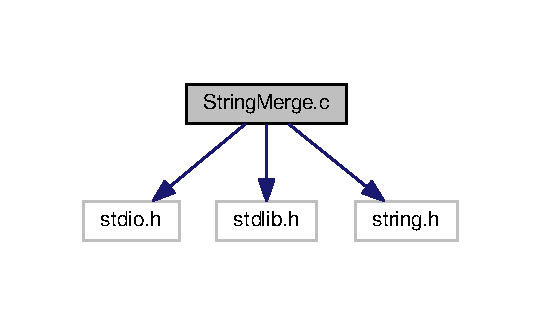
\includegraphics[width=260pt]{StringMerge_8c__incl}
\end{center}
\end{figure}
\subsection*{Macros}
\begin{DoxyCompactItemize}
\item 
\#define \hyperlink{StringMerge_8c_ab456f738bec038962389b5c5cfca3de4}{M\+A\+X\+B\+U\+F\+F\+ER}~128
\end{DoxyCompactItemize}
\subsection*{Functions}
\begin{DoxyCompactItemize}
\item 
int \hyperlink{StringMerge_8c_a1509289cc97c6ec0bad267f6c65fe0bf}{getlineE} (F\+I\+LE $\ast$fd, char buff\mbox{[}$\,$\mbox{]}, int nmax)
\item 
int \hyperlink{StringMerge_8c_aab69d82aeddb2aa4e003f7d03b975593}{string\+Merge} (char filename1\mbox{[}$\,$\mbox{]}, char filename2\mbox{[}$\,$\mbox{]}, char filename3\mbox{[}$\,$\mbox{]})
\item 
int \hyperlink{StringMerge_8c_a0ddf1224851353fc92bfbff6f499fa97}{main} (int argc, char $\ast$argv\mbox{[}$\,$\mbox{]})
\end{DoxyCompactItemize}


\subsection{Macro Definition Documentation}
\index{String\+Merge.\+c@{String\+Merge.\+c}!M\+A\+X\+B\+U\+F\+F\+ER@{M\+A\+X\+B\+U\+F\+F\+ER}}
\index{M\+A\+X\+B\+U\+F\+F\+ER@{M\+A\+X\+B\+U\+F\+F\+ER}!String\+Merge.\+c@{String\+Merge.\+c}}
\subsubsection[{\texorpdfstring{M\+A\+X\+B\+U\+F\+F\+ER}{MAXBUFFER}}]{\setlength{\rightskip}{0pt plus 5cm}\#define M\+A\+X\+B\+U\+F\+F\+ER~128}\hypertarget{StringMerge_8c_ab456f738bec038962389b5c5cfca3de4}{}\label{StringMerge_8c_ab456f738bec038962389b5c5cfca3de4}


\subsection{Function Documentation}
\index{String\+Merge.\+c@{String\+Merge.\+c}!getlineE@{getlineE}}
\index{getlineE@{getlineE}!String\+Merge.\+c@{String\+Merge.\+c}}
\subsubsection[{\texorpdfstring{getline\+E(\+F\+I\+L\+E $\ast$fd, char buff[], int nmax)}{getlineE(FILE *fd, char buff[], int nmax)}}]{\setlength{\rightskip}{0pt plus 5cm}int getlineE (
\begin{DoxyParamCaption}
\item[{F\+I\+LE $\ast$}]{fd, }
\item[{char}]{buff\mbox{[}$\,$\mbox{]}, }
\item[{int}]{nmax}
\end{DoxyParamCaption}
)}\hypertarget{StringMerge_8c_a1509289cc97c6ec0bad267f6c65fe0bf}{}\label{StringMerge_8c_a1509289cc97c6ec0bad267f6c65fe0bf}

\begin{DoxyCode}
12                                               \{
13   \textcolor{comment}{/* It reads a line from fd and stores up to nmax of 
}
14 \textcolor{comment}{   * its characters to buff.
}
15 \textcolor{comment}{   */}
16   \textcolor{keywordtype}{char} c;
17   \textcolor{keywordtype}{int} n=0;
18 
19   \textcolor{keywordflow}{while} ((c=getc(fd))!=\textcolor{charliteral}{'\(\backslash\)n'})\{
20     \textcolor{keywordflow}{if}(c==EOF)\textcolor{keywordflow}{return} EOF;
21     \textcolor{keywordflow}{if}(n<nmax)
22       buff[n++]=c;
23   \}
24   buff[n]=\textcolor{charliteral}{'\(\backslash\)0'};
25   \textcolor{keywordflow}{return} n;
26 \}
\end{DoxyCode}
\index{String\+Merge.\+c@{String\+Merge.\+c}!main@{main}}
\index{main@{main}!String\+Merge.\+c@{String\+Merge.\+c}}
\subsubsection[{\texorpdfstring{main(int argc, char $\ast$argv[])}{main(int argc, char *argv[])}}]{\setlength{\rightskip}{0pt plus 5cm}int main (
\begin{DoxyParamCaption}
\item[{int}]{argc, }
\item[{char $\ast$}]{argv\mbox{[}$\,$\mbox{]}}
\end{DoxyParamCaption}
)}\hypertarget{StringMerge_8c_a0ddf1224851353fc92bfbff6f499fa97}{}\label{StringMerge_8c_a0ddf1224851353fc92bfbff6f499fa97}

\begin{DoxyCode}
83                                  \{
84   \textcolor{keywordflow}{if}(argc!=4)\{
85     printf(\textcolor{stringliteral}{"Usage: %s sortedfile1 sortedfile2 mergefile\(\backslash\)n"}, argv[0]);
86     exit(0);
87   \}
88   printf(\textcolor{stringliteral}{"We have %d merged records\(\backslash\)n"},
89    \hyperlink{StringMerge_8c_aab69d82aeddb2aa4e003f7d03b975593}{stringMerge}(argv[1], argv[2], argv[3]));
90 \}
\end{DoxyCode}


Here is the call graph for this function\+:
\nopagebreak
\begin{figure}[H]
\begin{center}
\leavevmode
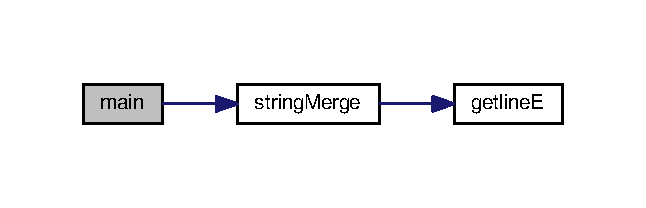
\includegraphics[width=310pt]{StringMerge_8c_a0ddf1224851353fc92bfbff6f499fa97_cgraph}
\end{center}
\end{figure}


\index{String\+Merge.\+c@{String\+Merge.\+c}!string\+Merge@{string\+Merge}}
\index{string\+Merge@{string\+Merge}!String\+Merge.\+c@{String\+Merge.\+c}}
\subsubsection[{\texorpdfstring{string\+Merge(char filename1[], char filename2[], char filename3[])}{stringMerge(char filename1[], char filename2[], char filename3[])}}]{\setlength{\rightskip}{0pt plus 5cm}int string\+Merge (
\begin{DoxyParamCaption}
\item[{char}]{filename1\mbox{[}$\,$\mbox{]}, }
\item[{char}]{filename2\mbox{[}$\,$\mbox{]}, }
\item[{char}]{filename3\mbox{[}$\,$\mbox{]}}
\end{DoxyParamCaption}
)}\hypertarget{StringMerge_8c_aab69d82aeddb2aa4e003f7d03b975593}{}\label{StringMerge_8c_aab69d82aeddb2aa4e003f7d03b975593}

\begin{DoxyCode}
28                                                                        \{
29   \textcolor{comment}{/* Given two sorted files of strings, called filename1 and filename2, 
}
30 \textcolor{comment}{   * it writes their merged sequence to the file filename3.
}
31 \textcolor{comment}{   * It returns the total number of strings written to filename3.
}
32 \textcolor{comment}{   */}
33   FILE *fd1, *fd2, *fd3;
34   \textcolor{keywordtype}{char} buffer1[\hyperlink{StringMerge_8c_ab456f738bec038962389b5c5cfca3de4}{MAXBUFFER}], buffer2[\hyperlink{StringMerge_8c_ab456f738bec038962389b5c5cfca3de4}{MAXBUFFER}];
35   \textcolor{keywordtype}{int} ln1, ln2;
36   \textcolor{keywordtype}{int} n=0;
37 
38   \textcolor{keywordflow}{if} ((fd1=fopen(filename1, \textcolor{stringliteral}{"r"}))==NULL) \{
39     perror(\textcolor{stringliteral}{"fopen"});
40     exit(1);
41   \}
42   \textcolor{keywordflow}{if} ((fd2=fopen(filename2, \textcolor{stringliteral}{"r"}))==NULL) \{
43     perror(\textcolor{stringliteral}{"fopen"});
44     exit(1);
45   \}
46   \textcolor{keywordflow}{if} ((fd3=fopen(filename3, \textcolor{stringliteral}{"w"}))==NULL) \{
47     perror(\textcolor{stringliteral}{"fopen"});
48     exit(1);
49   \}
50 
51   ln1 = \hyperlink{StringMerge_8c_a1509289cc97c6ec0bad267f6c65fe0bf}{getlineE}(fd1,buffer1,\hyperlink{StringMerge_8c_ab456f738bec038962389b5c5cfca3de4}{MAXBUFFER}-1);
52   ln2 = \hyperlink{StringMerge_8c_a1509289cc97c6ec0bad267f6c65fe0bf}{getlineE}(fd2,buffer2,\hyperlink{StringMerge_8c_ab456f738bec038962389b5c5cfca3de4}{MAXBUFFER}-1);
53 
54   \textcolor{keywordflow}{while} ((ln1!=EOF) && (ln2!=EOF))\{
55     \textcolor{keywordflow}{if} (strcmp(buffer1,buffer2)<=0)\{
56       fprintf(fd3, \textcolor{stringliteral}{"%s\(\backslash\)n"}, buffer1);
57       ln1 = \hyperlink{StringMerge_8c_a1509289cc97c6ec0bad267f6c65fe0bf}{getlineE}(fd1,buffer1,\hyperlink{StringMerge_8c_ab456f738bec038962389b5c5cfca3de4}{MAXBUFFER}-1);
58     \}\textcolor{keywordflow}{else}\{
59       fprintf(fd3, \textcolor{stringliteral}{"%s\(\backslash\)n"}, buffer2);
60       ln2 = \hyperlink{StringMerge_8c_a1509289cc97c6ec0bad267f6c65fe0bf}{getlineE}(fd2,buffer2,\hyperlink{StringMerge_8c_ab456f738bec038962389b5c5cfca3de4}{MAXBUFFER}-1);
61     \}
62     n++;
63   \}
64 
65   \textcolor{keywordflow}{while} (ln1!=EOF)\{
66       fprintf(fd3, \textcolor{stringliteral}{"%s\(\backslash\)n"}, buffer1);
67       ln1=\hyperlink{StringMerge_8c_a1509289cc97c6ec0bad267f6c65fe0bf}{getlineE}(fd1,buffer1,\hyperlink{StringMerge_8c_ab456f738bec038962389b5c5cfca3de4}{MAXBUFFER}-1);
68       n++;
69   \}
70 
71   \textcolor{keywordflow}{while} (ln2!=EOF)\{
72       fprintf(fd3, \textcolor{stringliteral}{"%s\(\backslash\)n"}, buffer2);
73       ln2=\hyperlink{StringMerge_8c_a1509289cc97c6ec0bad267f6c65fe0bf}{getlineE}(fd2,buffer2,\hyperlink{StringMerge_8c_ab456f738bec038962389b5c5cfca3de4}{MAXBUFFER}-1);
74       n++;
75   \}
76 
77   fclose(fd1);
78   fclose(fd2);
79   fclose(fd3);
80   \textcolor{keywordflow}{return} n;
81 \}
\end{DoxyCode}


Here is the call graph for this function\+:
\nopagebreak
\begin{figure}[H]
\begin{center}
\leavevmode
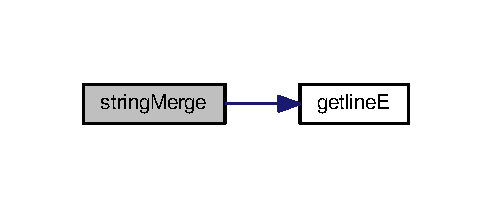
\includegraphics[width=236pt]{StringMerge_8c_aab69d82aeddb2aa4e003f7d03b975593_cgraph}
\end{center}
\end{figure}



%--- End generated contents ---

% Index
\backmatter
\newpage
\phantomsection
\clearemptydoublepage
\addcontentsline{toc}{chapter}{Index}
\printindex

\end{document}
